\documentclass{standalone}
\usepackage{bm}
\usepackage{amsmath}
\usepackage{amssymb}
\usepackage{dutchcal}
\usepackage{tikz}
\usetikzlibrary{decorations.pathmorphing}
\usetikzlibrary{decorations.markings}
\usetikzlibrary{patterns}
\usetikzlibrary{calc}
\usetikzlibrary{math}
\usetikzlibrary{fpu}
\usepackage{xcolor}
\definecolor{myGreen}{rgb}{0.2,0.72,0.2}
\definecolor{myWhite}{rgb}{0.98,0.98,0.98}
\definecolor{myGray}{rgb}{0.7,0.7,0.75}
\definecolor{myGold}{rgb}{0.8,0.64,0.24}

%%%%%%%%%%%%%%%%%%%%%CODE FROM INTERNET FOR GRID WITH COORDIATES%%%%
\makeatletter
\def\grd@save@target#1{%
  \def\grd@target{#1}}
\def\grd@save@start#1{%
  \def\grd@start{#1}}
\tikzset{
  grid with coordinates/.style={
    to path={%
      \pgfextra{%
        \edef\grd@@target{(\tikztotarget)}%
        \tikz@scan@one@point\grd@save@target\grd@@target\relax
        \edef\grd@@start{(\tikztostart)}%
        \tikz@scan@one@point\grd@save@start\grd@@start\relax
        \draw[minor help lines] (\tikztostart) grid (\tikztotarget);
        \draw[major help lines] (\tikztostart) grid (\tikztotarget);
        \grd@start
        \pgfmathsetmacro{\grd@xa}{\the\pgf@x/1cm}
        \pgfmathsetmacro{\grd@ya}{\the\pgf@y/1cm}
        \grd@target
        \pgfmathsetmacro{\grd@xb}{\the\pgf@x/1cm}
        \pgfmathsetmacro{\grd@yb}{\the\pgf@y/1cm}
        \pgfmathsetmacro{\grd@xc}{\grd@xa + \pgfkeysvalueof{/tikz/grid with coordinates/major step}}
        \pgfmathsetmacro{\grd@yc}{\grd@ya + \pgfkeysvalueof{/tikz/grid with coordinates/major step}}
        \foreach \x in {\grd@xa,\grd@xc,...,\grd@xb}
        \node[anchor=north] at (\x,\grd@ya) {\pgfmathprintnumber{\x}};
        \foreach \y in {\grd@ya,\grd@yc,...,\grd@yb}
        \node[anchor=east] at (\grd@xa,\y) {\pgfmathprintnumber{\y}};
      }
    }
  },
  minor help lines/.style={
    help lines,
    step=\pgfkeysvalueof{/tikz/grid with coordinates/minor step}
  },
  major help lines/.style={
    help lines,
    line width=\pgfkeysvalueof{/tikz/grid with coordinates/major line width},
    step=\pgfkeysvalueof{/tikz/grid with coordinates/major step}
  },
  grid with coordinates/.cd,
  minor step/.initial=.2,
  major step/.initial=1,
  major line width/.initial=2pt,
}
\newcommand{\Ds}{\displaystyle}

\begin{document}
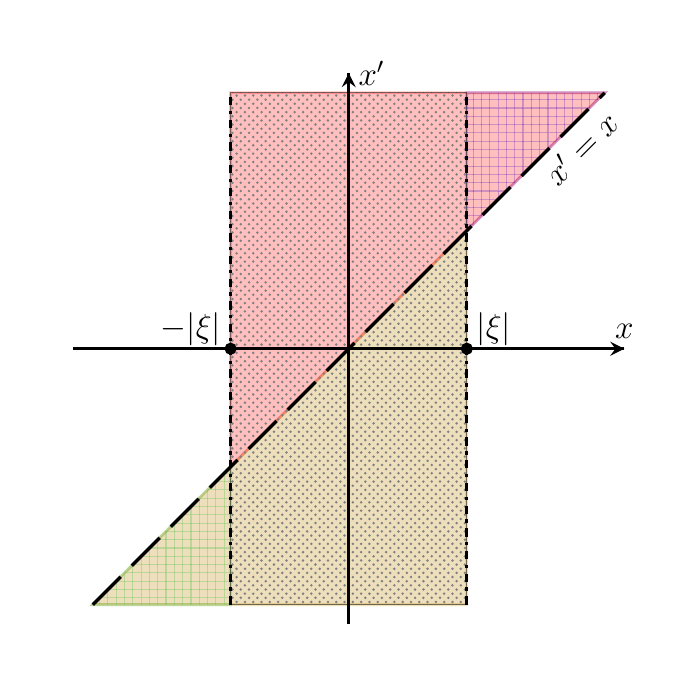
\begin{tikzpicture}
%\draw[step=.5cm] (-3,-3) to[grid with coordinates] (3,3);
\tikzmath{\s = 1.5;}

%%%%%%%%%%%%%%%%%%%%%%%%%%%%%%%%%%%%%%%%%%%%%%%%%%%%%%%%%%%%%% Setup
\coordinate (C) at (0, 0);
% just to have nice boundaries to the picture
\draw[white,fill=white] ($(-4,-4.0)$) circle (2pt);
\draw[white,fill=white] ($(+4,+4.0)$) circle (2pt);


%%%%%%%%%%%%%%%%%%%%%%%%%%%%%%%%%%%%%%%%%%%%%%%%%%%%%%%%%%%%%% Diag-1

% \xi = 1.5 for x\in[-4,4]
% \theta(x'-x)\theta(x-\xi)
\filldraw[draw=blue, fill=blue, line width=1pt,  draw opacity=0.25, pattern=grid, pattern color = blue] ($(C)+(1.5,1.5)$) -- ($(C)+(1.5,3.25)$) -- ($(C)+(3.25,3.25)$) -- cycle;

% \theta(-x'+x)\theta(-x+\xi)
\filldraw[draw=myGold, fill=myGold, line width=1pt, fill opacity=0.35, draw opacity=0.35] ($(C)+(1.5,1.5)$) -- ($(C)+(1.5,-3.25)$) -- ($(C)+(-3.25,-3.25)$) -- cycle;

% \theta(x'-x)\theta(x+\xi)
\filldraw[draw=red, fill=red, line width=1pt, fill opacity=0.25, draw opacity=0.25] ($(C)+(-1.5,-1.5)$) -- ($(C)+(-1.5,3.25)$) -- ($(C)+(3.25,3.25)$) -- cycle;

% \theta(-x'+x)\theta(-x-\xi)
\filldraw[draw=myGreen, fill=myGreen, line width=1pt,  draw opacity=0.25, pattern=grid, pattern color = myGreen] ($(C)+(-1.5,-1.5)$) -- ($(C)+(-1.5,-3.25)$) -- ($(C)+(-3.25,-3.25)$) -- cycle;

\draw[pattern={crosshatch dots}, pattern color = gray, draw opacity = 0.5] ($(C)+(-1.5,-3.25)$) -- ($(C)+(-1.5,3.25)$) -- ($(C)+(1.5,3.25)$) -- ($(C)+(1.5,-3.25)$) -- ($(C)+(-1.5,-3.25)$);

\draw[very thick, postaction={decorate, decoration={
    markings,
    mark=at position 1.0 with {\arrow{stealth}}}}] ($(C)+(-3.5,0)$)--($(C)+(3.5,0)$);
\draw[very thick, postaction={decorate, decoration={
    markings,
    mark=at position 1.0 with {\arrow{stealth}}}}] ($(C)+(0,-3.5)$)--($(C)+(0,3.5)$);

\draw[very thick, dash pattern=on 5mm off 2mm] ($(C)+(-3.25,-3.25)$)--($(C)+(3.25,3.25)$);

% -\xi
\draw[very thick, dash dot] ($(C)+(-1.5,-3.25)$)--($(C)+(-1.5,3.25)$);
% +\xi
\draw[very thick, dash dot] ($(C)+(1.5,-3.25)$)--($(C)+(1.5,3.25)$);
\node[above,right] at ($(C)+(0,3.5)$) {$\text{\large $x'$}$};
\node[above] at ($(C)+(3.5,0)$) {$\text{\large $x$}$};
\node[below, rotate=45] at ($(C)+(2.75,2.75)$) {$\text{\large $x'=x$}$};
\node[above,left] at ($(C)+(-1.5,0.25)$) {$\text{\large $-|\xi|$}$};
\node[above,right] at ($(C)+(1.5,0.25)$) {$\text{\large $|\xi|$}$};



\draw[black,fill=black] ($(C)+(-1.5,0)$) circle (2pt);
\draw[black,fill=black] ($(C)+(1.5,0)$) circle (2pt);



\end{tikzpicture}
\end{document}